\documentclass{beamer}

%
% Choose how your presentation looks.
%
% For more themes, color themes and font themes, see:
% http://deic.uab.es/~iblanes/beamer_gallery/index_by_theme.html
%
\mode<presentation>
{
  \usetheme{default}      % or try Darmstadt, Madrid, Warsaw, ...
  \usecolortheme{default} % or try albatross, beaver, crane, ...
  \usefonttheme{default}  % or try serif, structurebold, ...
  \setbeamertemplate{navigation symbols}{}
  \setbeamertemplate{caption}[numbered]
  \setbeamertemplate{footline}[page number]
  \setbeamercolor{frametitle}{fg=white}
  \setbeamercolor{footline}{fg=black}
} 

\usepackage[english]{babel}
\usepackage[utf8x]{inputenc}
\usepackage{tikz}
\usepackage{listings}
\usepackage{courier}
\usepackage{minted}
\usepackage{array}

\xdefinecolor{darkblue}{rgb}{0.1,0.1,0.7}
\xdefinecolor{darkgreen}{rgb}{0,0.5,0}
\xdefinecolor{darkorange}{rgb}{0.8,0.5,0}
\xdefinecolor{darkred}{rgb}{0.7,0,0}
\xdefinecolor{dianablue}{rgb}{0.18,0.24,0.31}
\definecolor{commentgreen}{rgb}{0,0.6,0}
\definecolor{stringmauve}{rgb}{0.58,0,0.82}

\lstset{ %
  backgroundcolor=\color{white},      % choose the background color
  basicstyle=\ttfamily\small,         % size of fonts used for the code
  breaklines=true,                    % automatic line breaking only at whitespace
  captionpos=b,                       % sets the caption-position to bottom
  commentstyle=\color{commentgreen},  % comment style
  escapeinside={\%*}{*)},             % if you want to add LaTeX within your code
  keywordstyle=\color{blue},          % keyword style
  stringstyle=\color{stringmauve},    % string literal style
  showstringspaces=false,
  showlines=true
}

\lstdefinelanguage{scala}{
  morekeywords={abstract,case,catch,class,def,%
    do,else,extends,false,final,finally,%
    for,if,implicit,import,match,mixin,%
    new,null,object,override,package,%
    private,protected,requires,return,sealed,%
    super,this,throw,trait,true,try,%
    type,val,var,while,with,yield},
  otherkeywords={=>,<-,<\%,<:,>:,\#,@},
  sensitive=true,
  morecomment=[l]{//},
  morecomment=[n]{/*}{*/},
  morestring=[b]",
  morestring=[b]',
  morestring=[b]"""
}

\title[2016-12-16-femtocode-overview]{Femtocode Overview}
\author{Jim Pivarski}
\institute{Princeton University -- DIANA}
\date{December 16, 2016}

\begin{document}

\logo{\pgfputat{\pgfxy(0.11, 8)}{\pgfbox[right,base]{\tikz{\filldraw[fill=dianablue, draw=none] (0 cm, 0 cm) rectangle (50 cm, 1 cm);}}}\pgfputat{\pgfxy(0.11, -0.6)}{\pgfbox[right,base]{\tikz{\filldraw[fill=dianablue, draw=none] (0 cm, 0 cm) rectangle (50 cm, 1 cm);}
\includegraphics[height=0.99 cm]{diana-hep-logo.png}\tikz{\filldraw[fill=dianablue, draw=none] (0 cm, 0 cm) rectangle (4.9 cm, 1 cm);}}}}

\begin{frame}
  \titlepage
\end{frame}

\logo{\pgfputat{\pgfxy(0.11, 8)}{\pgfbox[right,base]{\tikz{\filldraw[fill=dianablue, draw=none] (0 cm, 0 cm) rectangle (50 cm, 1 cm);}
\includegraphics[height=1 cm]{diana-hep-logo.png}}}}

% Uncomment these lines for an automatically generated outline.
%\begin{frame}{Outline}
%  \tableofcontents
%\end{frame}

% HERE HERE HERE HERE HERE HERE HERE HERE HERE HERE HERE HERE HERE HERE HERE

\begin{frame}{Essential and accidental complexity}
\vspace{0.25 cm}
\textcolor{darkorange}{\bf End-user physics analysis \underline{must} include the following:}
\begin{description}
\item[\bf big data pull:] probably with on-the-fly filters and transformations, given the scale of the data,
\item[\bf manipulations:] at least plotting, but probably fitting, unfolding, cross-comparisons, machine learning, etc.
\end{description}

\vfill
\begin{uncoverenv}<2->
\textcolor{darkorange}{\bf Currently, most analyses also include:}
\begin{description}
\item[\bf private skim:] intermediate-sized dataset with more fields than necessary.
\begin{itemize}
\item Since the big data pull takes so long, fields that {\it might} be needed are included as a hedge.
\item This makes the big data pull bigger.

\textcolor{gray}{(The more skim you have, the more you need!)}
\end{itemize}
\end{description}
\end{uncoverenv}
\end{frame}

\begin{frame}{Reducing dataset size early}
\begin{center}
\only<1>{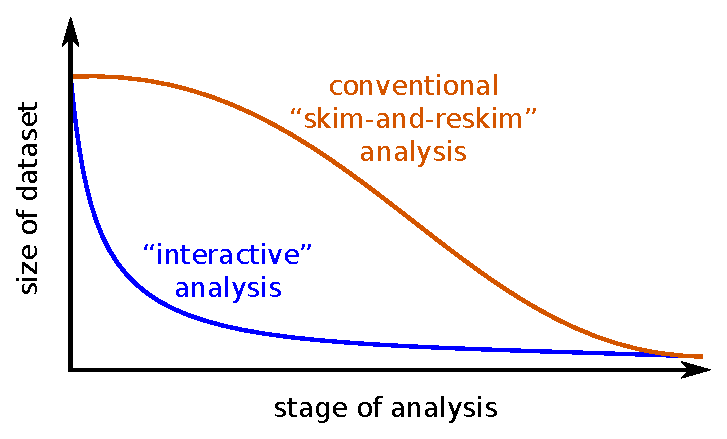
\includegraphics[width=0.8\linewidth]{pseudoplot.pdf}}
\only<2>{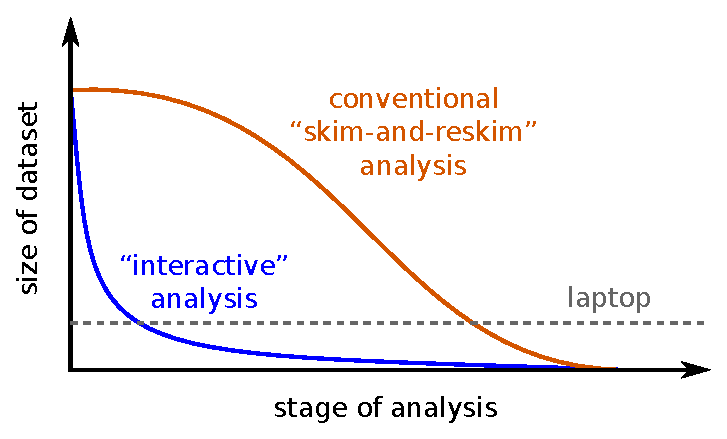
\includegraphics[width=0.8\linewidth]{pseudoplot2.pdf}}
\end{center}

Ideally, data should go directly from the collaboration-wide store (e.g.\ MiniAOD) into plots, fits, or machine learning algorithms, rapidly enough that there's no temptation to overstock the big data pull.
\end{frame}

\begin{frame}{Industry {\it expects} interactive analysis}

Business intelligence has traditionally been interactive; there's a race to provide interactivity with Big Data backends:

\begin{center}
\textcolor{blue}{Ibis, Impala, Kudu, Drill, \ldots}
\end{center}

all aim to yield sub-second results from terabytes or petabytes of data. (And Google claims to have had it, in-house, for ten years: see \href{http://research.google.com/pubs/pub36632.html}{\textcolor{blue}{Dremel paper}}.)

\vfill
\textcolor{darkorange}{\bf Shouldn't we?}
\end{frame}

\begin{frame}{How could this even be possible?}
\vspace{0.5 cm}
\textcolor{darkorange}{\bf How could a week-long GRID job be reduced to seconds?}

\vspace{0.5 cm}
\begin{columns}[t]
\column{0.5\linewidth}
\textcolor{darkblue}{\underline{\bf GRID job}}

\begin{itemize}
\item Includes data fields that {\it might} be useful.

\item Framework reconstructs whole C++ objects, regardless of whether they're split in ROOT: loading {\it dozens} of unused fields.

\item Bad choices in user's C++.

\item Finding storage for and moving the big output files.
\end{itemize}

\column{0.5\linewidth}
\textcolor{darkblue}{\underline{\bf Interactive query}}

\begin{itemize}
\item Limited to fields mentioned in the query.

\item Only loads the attributes mentioned in the query: rarely more than 5--10.

\item Can employ JIT or other optimizations.

\item Can cache frequently requested fields or subexpressions among users.
\end{itemize}
\end{columns}

\vspace{0.5 cm}
\textcolor{gray}{(Not to mention {\it user's time} needed to write and test the code.)}
\end{frame}

\begin{frame}{How could this even be possible?}
\vspace{0.5 cm}
\large \textcolor{darkblue}{\underline{Numbers for sanity check:}}
\begin{itemize}
\item 2010--2016 CMS data is about 100~fb$^{-1}$ (\href{http://cms-service-lumi.web.cern.ch/cms-service-lumi/publicplots/int_lumi_cumulative_pp_1.png}{\textcolor{blue}{plot}}),
\item $t\bar{t}$ is 1000~pb (\href{https://atlas.web.cern.ch/Atlas/GROUPS/PHYSICS/CombinedSummaryPlots/SM/ATLAS_p_SMSummary_SqrtS_Zoom/ATLAS_p_SMSummary_SqrtS_Zoom.png}{\textcolor{blue}{plot}}),
\item say you want to look at 100 numerical values per event,
\item 8 bytes per double-precision value,
\end{itemize}
that's 80~GB of data to examine, with all overhead eliminated.

\vspace{0.5 cm}
\uncover<2->{That could take seconds to minutes to analyze on a single computer, depending.}

\vspace{0.2 cm}
\uncover<3->{3.2 seconds to copy to GPU and 0.16 seconds to analyze on a single computer with a typical (Tesla K20) GPU.}

\vspace{0.2 cm}
\uncover<4->{This embarrassingly parallel problem can be distributed across a cluster of servers.}
\end{frame}

\begin{frame}{}
\begin{center}
\textcolor{darkblue}{\huge But\ldots}
\end{center}
\end{frame}

\begin{frame}[fragile]{Physics data are different}
\vspace{0.5 cm}
Most datasets in industry are (the equivalent of) flat ntuples:
\begin{itemize}
\item SQL tables
\item OLAP hypercubes
\item exceptions are often handled with user-defined functions
(e.g.\ lat, lon $\to$ zip code, followed by ntuple analysis on zip codes).
\end{itemize}

\vfill
\begin{uncoverenv}<2->
Modern SQL engines are capable of nested structure, but have no functions for dealing with the structure other than exploding it.

\vspace{0.25 cm}
\textcolor{darkblue}{Physics equivalent:} doing all analysis with TTreeFormula:

\begin{lstlisting}[language=c]
ntuple->Draw("tracks[].hits[].residual >> hresid");
\end{lstlisting}
\end{uncoverenv}
\end{frame}

\begin{frame}{Physics data are different}
\vspace{0.25 cm}
{\bf Spark has two options:}
\begin{enumerate}
\item SQL-style analysis with DataFrames \textcolor{gray}{(Column expressions)},
\item General analysis with RDDs \textcolor{gray}{(any Scala or Python function)}.
\end{enumerate}
When I asked Michael Armbridge (Databricks) about this, he said the goal of DataFrames was to ``cover 95\% of the use-cases.''

\vfill
Physics analysis with flat ntuples is within their ``95\%,'' but something like this isn't:
\begin{center}
\begin{minipage}{0.95\linewidth}
\textcolor{darkblue}{``Momentum of the track with $|\eta|$ $<$ 2.4 that has the most hits.''}
\end{minipage}
\end{center}

\vfill
Restricting to flat ntuple analysis would require more skims. Spark solves the bookkeeping aspects, but not the fundamental problem.
\end{frame}

\begin{frame}{We need expressiveness {\it and} optimizability}
\vspace{0.5 cm}
\begin{center}
\begin{minipage}{0.9\linewidth}
To replace GRID jobs with declarative queries, the query \mbox{language} must be
\begin{itemize}
\item \textcolor{darkblue}{\it more expressive} than SQL and TTreeFormula,
\item \textcolor{darkblue}{\it less expressive} than code (to permit optimizations and subexpression caching, like Spark's DataFrames).
\end{itemize}

\vspace{0.5 cm}
Nothing exists to fill this gap.

\textcolor{gray}{(For most of this year, I've been looking.)}

\vspace{0.5 cm}
Need to invent a query language: \textcolor{darkblue}{Femtocode}.
\end{minipage}
\end{center}
\end{frame}

\begin{frame}[fragile]{Nested query in SQL}
\vspace{0.25 cm}
\begin{center}
\begin{minipage}{0.95\linewidth}
\textcolor{darkblue}{``Momentum of the track with $|\eta|$ $<$ 2.4 that has the most hits.''}
\end{minipage}
\end{center}
\small
\begin{minted}{sql}
WITH hit_stats AS (
  SELECT hit.track_id, COUNT(*) AS hit_count FROM hit
    GROUP BY hit.track_id),
 track_sorted AS (
    SELECT track.*, 
    ROW_NUMBER() OVER (
     PARTITION BY track.event_id
     ORDER BY hit_stats.hit_count DESC)
  track_ordinal FROM track INNER JOIN hit_stats
    ON hit_stats.track_id = track.id
    WHERE ABS(track.eta) < 2.4)
 SELECT * FROM event INNER JOIN track_sorted
   ON track_sorted.event_id = event.id
WHERE
  track_sorted.track_ordinal = 1
\end{minted}
\end{frame}

\begin{frame}[fragile]{Nested query in C++}
\vspace{0.25 cm}
\begin{center}
\begin{minipage}{0.95\linewidth}
\textcolor{darkblue}{``Momentum of the track with $|\eta|$ $<$ 2.4 that has the most hits.''}
\end{minipage}
\end{center}
\small
\begin{minted}{c++}
Track *best = NULL;
for (int i = 0;  i < tracks.size();  i++) {
  if (fabs(tracks[i]->eta) < 2.4)
    if (best == NULL ||
        tracks[i]->hits.size() < best->hits.size())
      best = tracks[i];
}
if (best != NULL)
  return best->pt;
else
  return 0.0;
\end{minted}
\end{frame}

\begin{frame}[fragile]{Nested query in Femtocode}
\vspace{0.25 cm}
\begin{center}
\begin{minipage}{0.95\linewidth}
\textcolor{darkblue}{``Momentum of the track with $|\eta|$ $<$ 2.4 that has the most hits.''}
\end{minipage}
\end{center}
\small
\begin{onlyenv}<1>
\begin{minted}{scala}
event.tracks
     .filter(t => abs(t.eta) < 2.4)
     .maxBy(t => t.hits.size)
     .map(t => t.pt)
     .impute(0.0)
\end{minted}
\end{onlyenv}
\begin{onlyenv}<2>
\begin{minted}{bash}
event.tracks
     .filter(abs($1.eta) < 2.4)
     .maxBy($1.hits.size)
     .map($1.pt)
     .impute(0.0)
\end{minted}
\end{onlyenv}
\end{frame}

\begin{frame}{Features of Femtocode}
\vspace{0.5 cm}
\begin{description}
\item[Declarative:]<1-> order written/order evaluated need not be the same.
\item[Functional:]<2-> map/filter/maxBy instead of explicit for loops.
\item[Vectorizable:]<3-> code appears to act on rows (e.g.\ events), but automatically translated to operate on columns.
\item[No unbounded loops:]<4-> execution time strictly scales with input data size; not Turing complete.
\item[No runtime errors:]<5-> any compilable query will return some result.
\item[Statically typed:]<6-> stronger type system than most languages is needed to eliminate runtime errors.
\item[Full type inference:]<7-> explicitly writing down types is annoying.
\item[No recursion:]<8-> combining recursion with \textcolor{darkblue}{no unbounded loops} is complicated, but big data pulls don't need recursion.
\item[Pythonic syntax:]<9-> familiar to physics users; don't invent new syntax unless absolutely necessary.
\end{description}
\end{frame}

\begin{frame}[fragile]{High-level overview}
\vspace{0.5 cm}
Femtocode transforms datasets into
\begin{itemize}
\item other datasets \textcolor{gray}{(can be virtual/intermediate, not stored)},
\item flat tables of numbers \textcolor{gray}{(for unbinned fits/machine learning)},
\item Histogrammar aggregations \textcolor{gray}{(broad class of aggregations)}.
\end{itemize}

It is used only for the \textcolor{darkblue}{\bf big data pull}, not the \textcolor{darkblue}{\bf manipulations}.

\vspace{0.5 cm}
\begin{uncoverenv}<2->
\textcolor{darkorange}{\bf \underline{Example use:}}

\small
\begin{minted}{python}
h = db.dataset("ttbar-MC")
  .withColumn(varName = "<Femtocode goes here>")
  .filter("<Femtocode using varName>")
  .flatMap("<Femtocode changing nesting level>")
  .Label(hist1 = Bin(100, -5.0, 5.0, "<Femtocode>"),
         hist2 = Bin(20, 0.0, 100.0, "<Femtocode>"),
         hist3 = Bin(314, -pi, pi, "<Femtocode>"))
\end{minted}

\normalsize
followed by Python analysis with {\small\tt h[\textcolor{darkred}{"hist1"}]}, {\small\tt h[\textcolor{darkred}{"hist2"}]}\ldots
\end{uncoverenv}
\end{frame}

\begin{frame}{What is a dataset?}
\vspace{0.25 cm}
\begin{center}
\begin{minipage}{0.9\linewidth}
\textcolor{darkorange}{\bf An unordered collection of named, typed values.}

\vspace{0.25 cm}
For instance, events characterized by a set of measurements.
\end{minipage}
\end{center}

\begin{uncoverenv}<2->
Many concrete realizations:
\begin{itemize}
\item \textcolor{darkblue}{Terascope server:} responds to user queries with aggressive optimizations. Goal is sub-second response.
\item \textcolor{darkblue}{ROOT TTrees:} integrates with ROOT team's efforts at functional chains; Femtocode may become the ROOT 7 TTreeFormula.
\item \textcolor{darkblue}{GPU:} Femtocode's vectorizability fits perfectly into the GPU's SIMD architecture; special optimization for \textcolor{darkblue}{Terascope server}.
\item \textcolor{darkblue}{Spark:} extend the usability of Spark's DataFrames.
\item \textcolor{darkblue}{Apache Arrow:} target many big data platforms at once.
\end{itemize}
\end{uncoverenv}
\end{frame}

\begin{frame}{What is a dataset?}
\vspace{0.5 cm}
\textcolor{darkblue}{\large Alternate definition:}

\vspace{0.2 cm}
\mbox{ } \hfill \textcolor{darkorange}{\bf A dataset is a mapping from schema leaves to columns.} \hfill \mbox{ }

\vspace{0.5 cm}
\begin{columns}
\column{0.5\linewidth}
Even if the schema has nested structure, it is possible to write each schema leaf (primitive type) as an array of primitives.

\vspace{0.2 cm}
Some arrays would be longer than others.

\column{0.4\linewidth}
\vspace{-0.4 cm}
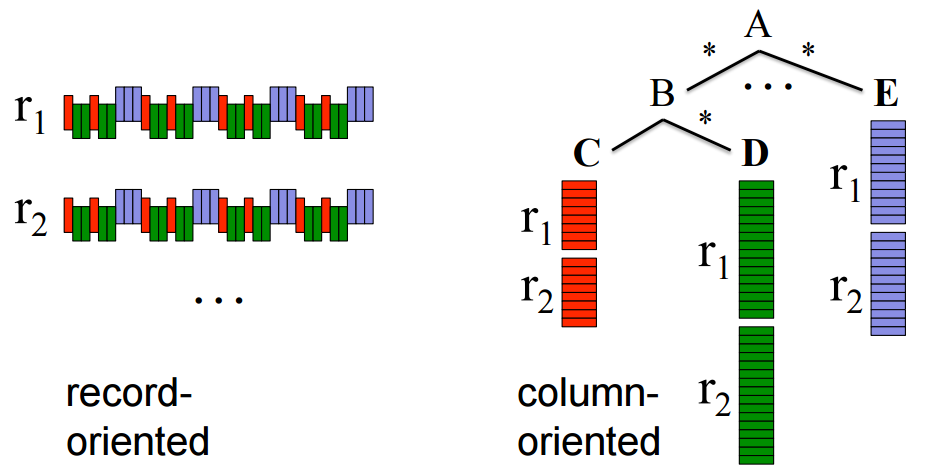
\includegraphics[width=\linewidth]{columnar.png}
\end{columns}

\vspace{0.5 cm}
\begin{center}
\large \textcolor{darkblue}{Different versions of a dataset can share all but one leaf.}

\vspace{0.4 cm}
\normalsize Very lightweight updates: correcting an error in jet energy scale doesn't need to affect track parameters (for instance).
\end{center}
\end{frame}

\begin{frame}{Updating datasets (e.g.\ in CMS)}
\small
\vspace{0.5 cm}
\textcolor{darkblue}{Central reprocessing, replace all:}
\vspace{-0.15 cm}
\begin{enumerate}\setlength{\itemsep}{-0.1 cm}
\item \small CMS runs CMSSW, produces new data products in ROOT files,
\item \small data products are converted into columns,
\item \small new dataset names associated with new columns.
\end{enumerate}

\textcolor{darkblue}{Central bug-fix, replacing a few values:}
\vspace{-0.15 cm}
\begin{enumerate}\setlength{\itemsep}{-0.1 cm}
\item \small CMS runs CMSSW, produces only the new data products in \mbox{ROOT files,\hspace{-1 cm}}
\item \small only new data products are converted into columns,
\item \small new dataset names associated with old and new columns.
\end{enumerate}

\textcolor{darkblue}{User wants to share derived quantity from CMSSW:}
\vspace{-0.15 cm}
\begin{enumerate}\setlength{\itemsep}{-0.1 cm}
\item \small User runs CMSSW, produces only the new data products in \mbox{ROOT files,\hspace{-1 cm}}
\item \small only new data products are converted into columns,
\item \small new dataset names associated with old and new columns.
\end{enumerate}

\textcolor{darkblue}{User wants to share derived quantity from Femtocode:}
\vspace{-0.15 cm}
\begin{enumerate}\setlength{\itemsep}{-0.1 cm}
\item \small User runs Femtocode, saves and names new column,
\item \small new dataset name associated with old and new columns.
\end{enumerate}

\textcolor{darkblue}{Implicit sharing:}
\vspace{-0.15 cm}
\begin{enumerate}\setlength{\itemsep}{-0.1 cm}
\item \small Frequently calculated subexpressions can be implicitly cached.
\end{enumerate}
\end{frame}

\begin{frame}{Cross-references}
The Femtocode type system (next page) has no ``pointers,'' no way to make a reference within the event.

\vspace{0.2 cm}
\textcolor{gray}{(For instance, for a muon object to point to its track or a jet object to point to its collection of tracks.)}

\vspace{0.5 cm}
However, Femtocode also has value-equality: no distinction between copying and referencing. Backend can present ``virtual columns,'' indexes into some other collection, as nested data.

\vspace{0.5 cm}
\textcolor{gray}{(Thus, the distinction between a muon {\it pointing} to its track and containing a {\it copy} of its track is a backend optimization, not visible to the Femtocode user.)}
\end{frame}

\begin{frame}{Abstract type system}
\vspace{0.5 cm}
Space of possible datasets is defined by the type system.

\begin{description}
\item[null:] type with only one value
\item[boolean:] not the same as integers
\item[number:] further defined by attributes: \textcolor{darkblue}{min}, \textcolor{darkblue}{max}, \textcolor{darkblue}{whole}

{\tt whole == True} means integer,

{\tt whole == False} means floating point

\item[string:] \textcolor{darkblue}{charset} (``bytes'' or ``unicode''), \textcolor{darkblue}{fewest}, \textcolor{darkblue}{most};

\textcolor{darkblue}{fewest/most} constrain the string length

\item[collection:] \textcolor{darkblue}{fewest}, \textcolor{darkblue}{most}, \textcolor{darkblue}{ordered}

fixed-size arrays/matrices have {\tt fewest == most and ordered == True}

\item[record:] defined by a dictionary of \textcolor{darkblue}{fields}
\item[union:] tagged union, such as {\tt union(null, string)} for a nullable string type.
\end{description}
\end{frame}

\begin{frame}[fragile]{This is a high-granularity type system}
\vspace{0.5 cm}
The ``number'' type has \textcolor{darkblue}{min} and \textcolor{darkblue}{max} attributes, and these can be open or closed intervals.
\begin{itemize}
\item {\tt real(almost(0), 10)} means $\{x | x \in \mathbb{R}\mbox{ and } 0 < x \le 10\}$
\item {\tt integer(almost(-inf), almost(inf))} means $\mathbb{Z}$
\item {\tt extended(-inf, inf)} means $\mathbb{R} \cup \{-\infty, \infty\}$
\item {\tt union(integer, real(0))} means

\hfill $\mathbb{Z} \cup \{x | x \in \mathbb{R}\mbox{ and } x \ge 0\}$
\end{itemize}

\vfill
\begin{uncoverenv}<2->
\textcolor{darkorange}{\bf Why?}

The type system has to know enough to eliminate the possibility of runtime error.

\vspace{0.2 cm}
\textcolor{darkorange}{\bf Example}

If {\tt x} and {\tt y} are {\tt real}, then ``{\tt x/y}'' is a type error but

\vspace{0.2 cm}
\mbox{ } \hfill ``{\tt if y != 0:\ x/y else:\ None}'' \hfill \mbox{ }

\vspace{0.2 cm}
is legal. The error message directs the user to fix their code.
\end{uncoverenv}
\end{frame}

\begin{frame}{Type inference}
\vspace{0.3 cm}
\textcolor{darkorange}{\bf Same example}

If {\tt x} and {\tt y} are {\tt real},

\vspace{0.2 cm}
\mbox{ } \hfill ``{\tt if y != 0:\ x/y else:\ None}'' \hfill \mbox{ }

\vspace{0.2 cm}
illustrates the flow of type inference.

\vspace{0.3 cm}
\begin{uncoverenv}<2->
Starts with input dataset schema fields ({\tt x} and {\tt y}), propagates from function arguments to return type.
\end{uncoverenv}

\vspace{0.3 cm}
\begin{uncoverenv}<3->
``if'' predicates, as well as ``and'' and ``or'' conjunctions, constrict the data type of a variable, in this case from {\tt real} to

\mbox{\tt union(real(max=almost(0)), real(min=almost(0)))}.
\end{uncoverenv}

\begin{uncoverenv}<4->
\vspace{-0.2 cm}
Inside the {\tt else} clause, {\tt y} can have only one value: {\tt real(0, 0)}.
\end{uncoverenv}

\begin{uncoverenv}<5->
\vspace{-0.2 cm}
The resulting type of the whole expression is {\tt union(null, extended)}. This would raise a type error if the user tried to insert it into a function that doesn't accept {\tt None}, or {\tt inf} (e.g.\ {\tt sin} and {\tt cos}), or negative values (e.g.\ {\tt sqrt}).
\end{uncoverenv}
\end{frame}

\begin{frame}{Logical inference}
\vspace{0.25 cm}
Perhaps this looks like a formal proof system or a computer algebra system. In a way, every type-checker is (Curry-Howard correspondence).

\vspace{0.25 cm}
\begin{uncoverenv}<2->
\textcolor{darkblue}{Femtocode has just enough type system granularity to eliminate runtime errors:}
\begin{itemize}
\item unions of intervals of numbers,
\item string and collection size bounds (avoid index overflows),
\item interval propagation through {\tt +}, {\tt -}, {\tt *}, {\tt /}, {\tt //}, {\tt **}, {\tt \%}, and numerical functions (e.g.\ {\tt sin}, {\tt cos}, {\tt sqrt}),
\item no attempt to track correlations, like {\tt x - y} having a smaller interval than {\tt x} and {\tt y} separately,
\item structural record types (records are the same if they have the same fields),
\item user-defined functions are taken to be parametric in all parameters (so that logical inference always flows in one direction).
\end{itemize}
\end{uncoverenv}
\end{frame}

\begin{frame}{}
\begin{center}
\textcolor{darkblue}{\huge Syntax}
\end{center}
\end{frame}

\begin{frame}[fragile]{Syntax}
\vspace{0.25 cm}
\textcolor{darkblue}{BNF specification of Femtocode syntax} \only<2->{\textcolor{red}{that is identical to Python}}

\vspace{-0.5 cm}
\begin{columns}[t]
\column{0.5\linewidth}
\tiny
\begin{verbatim}
body: ';'* suite
suite: (assignment ';'*)* expression ';'*
lvalues: (NAME ',')* NAME [',']
assignment: (lvalues '=' closed_expression
              | fcnndef)
fcnndef: ('def' NAME '(' [paramlist] ')'
            closed_exprsuite)
expression: ifblock | fcndef | or_test
closed_expression: (closed_ifblock | fcndef
                     | or_test ';')
fcndef: '{' [paramlist] '=>' ';'* suite '}'
fcn1def: parameter '=>' expression
paramlist: (parameter ',')* (parameter [','])
parameter: NAME ['=' expression]
exprsuite: (':' expression
             | [':'] '{' ';'* suite '}')
closed_exprsuite: (':' closed_expression
             | [':'] '{' ';'* suite '}')
ifblock: ('if' expression exprsuite
            ('elif' expression exprsuite)*
             'else' exprsuite)
closed_ifblock: ('if' expression exprsuite
            ('elif' expression exprsuite)*
             'else' closed_exprsuite)
\end{verbatim}
\vspace{-0.8 cm}\only<2->{\color{red}}
\begin{verbatim}
or_test: and_test ('or' and_test)*
and_test: not_test ('and' not_test)*
not_test: 'not' not_test | comparison
comparison: typecheck (comp_op typecheck)*
comp_op: ('<' | '>' | '==' | '>=' | '<='
              | '!=' | 'in' | 'not' 'in')
\end{verbatim}

\column{0.5\linewidth}
\tiny\only<2->{\color{black}}
\begin{verbatim}
typecheck: (arith_expr ['is' arith_expr
             | 'is' 'not' arith_expr])
\end{verbatim}
\vspace{-0.8 cm}\only<2->{\color{red}}
\begin{verbatim}
arith_expr: term (('+' | '-') term)*
term: factor (('*' | '/' | '%' | '//') factor)*
factor: ('+' | '-') factor | power
power: atom trailer* ['**' factor]
atom: ('(' expression ')'
\end{verbatim}
\vspace{-0.8 cm}\only<2->{\color{black}}
\begin{verbatim}
       | ('[' (expression ',')*
             [expression [',']] ']')
       | fcndef '(' [arglist] ')'
\end{verbatim}
\vspace{-0.8 cm}\only<2->{\color{red}}
\begin{verbatim}
       | MULTILINESTRING
       | STRING
       | IMAG_NUMBER
       | FLOAT_NUMBER
       | HEX_NUMBER
       | OCT_NUMBER
       | DEC_NUMBER
\end{verbatim}
\vspace{-0.8 cm}\only<2->{\color{black}}
\begin{verbatim}
       | ATARG
\end{verbatim}
\vspace{-0.8 cm}\only<2->{\color{red}}
\begin{verbatim}
       | NAME)
trailer: ('(' [arglist] ')'
           | '[' subscriptlist ']' | '.' NAME)
subscriptlist: subscript (',' subscript)* [',']
subscript: (expression
           | [expression] ':' [expression]
             [sliceop])
sliceop: ':' [expression]
\end{verbatim}
\vspace{-0.8 cm}\only<2->{\color{black}}
\begin{verbatim}
arglist: (((argument ',')* (argument [',']))
           | fcn1def)
argument: expression | NAME '=' expression
\end{verbatim}
\end{columns}
\end{frame}

\begin{frame}[fragile]{Syntax}
\vspace{0.3 cm}
\begin{columns}[t]
\column{0.5\linewidth}
\textcolor{darkblue}{\underline{\bf How is it like Python?}}
\begin{itemize}
\item mathematical expressions and operator precedence:

{\small\tt (-b + sqrt(b**2 -

\hfill 4*a*c))/(2*a)}

\item slices and 0-indexing:

{\small\tt lheweights[::2]}

\item numbers and string literals (favoring Python 3):

{\small\tt 0xff, 0o77, .3e7, 1j,

"""multi \textbackslash"line\textbackslash"

string"""}

\item chained comparisons:

{\small\tt 0 < x <= 10}

\item keyword arguments:

{\small\tt f(arg, some=kwd)}

\end{itemize}

\column{0.5\linewidth}
\textcolor{darkblue}{\underline{\bf How is it different?}}
\begin{itemize}
\item anonymous functions:

{\small\tt \{x, y => x + y\}

\{\$1 + \$2\}}

\item no statements and whitespace independent:

{\small\tt if something:

\ \ \ doIfTrue()

\ \ \ else:

\ doIfFalse()}

\item curly-bracketed blocks with semicolon-separated assignments ending in a single expression.

{\small\tt if something \{doIfTrue()\} else \{doIfFalse()\}}
\end{itemize}
\end{columns}
\end{frame}

\begin{frame}{Syntax summary}
\vspace{0.5 cm}
\textcolor{darkblue}{Users should approach Femtocode as a new language.}

\vspace{0.5 cm}
However, the things they don't think about (e.g.\ operator precedence) offer no surprises if they're coming from Python.

\vspace{0.5 cm}
\uncover<2->{Whitespace independence and rules involving curly brackets and semicolons work like C, so that shouldn't be surprising, either.}

\vspace{0.5 cm}
\uncover<3->{Arrow operators to define functions (e.g.\ {\tt \{x, y => x + y\}}) are pretty common, too: C\#, Scala, Javascript 6+, Coffeescript, \ldots}

\vspace{0.5 cm}
\uncover<4->{Anonymous function shorthand (e.g.\ {\tt \{\$1 + \$2\}}) is inspired by Scala's underscores, but using bash dollar signs for familiarity.}
\end{frame}

\begin{frame}{}
\begin{center}
\textcolor{darkblue}{\huge Semantics}
\end{center}
\end{frame}

\begin{frame}{Semantics}
Every Femtocode ``program'' is conceptually a single expression: that which should be computed from the input fields.
\begin{itemize}
\item when called in a {\tt filter}, it selects events,
\item in {\tt map}, it transforms,
\item in {\tt flatMap}, it restructures,
\item in {\tt withColumn}, it adds a field to the output,
\item in Histogrammar quantities, it gets aggregated, probably for plotting.
\end{itemize}

\vspace{0.5 cm}
Most Femtocode snippets are small enough for this to be obvious!
\end{frame}

\begin{frame}[fragile]{Semantics}
\vspace{0.5 cm}
Assignments are provided {\it as a convenience.}

\begin{center}
\begin{minipage}{0.9\linewidth}
\small
\begin{lstlisting}[language=python]
goodVertex = abs(z) < 3;
goodPt = pt > 20;
goodIsolation = iso > 12;
goodVertex and goodPt and goodIsolation
\end{lstlisting}
\end{minipage}
\end{center}

Expression ASTs are literally inserted where they are referenced \textcolor{gray}{(handling shadowed variable names appropriately, with lexical scope)}.

\vspace{0.5 cm}
This is legal because Femtocode has perfect referential transparency. \textcolor{gray}{(All variables are immutable, no side-effects, no exceptions or non-halting functions.)}
\end{frame}

\begin{frame}[fragile]{Semantics}
\vspace{0.5 cm}
The same is true of user-defined functions. Moreover, arguments might have different types in different calls.

\begin{center}
\begin{minipage}{0.9\linewidth}
\small
\begin{lstlisting}[language=python]
def nonempty(x) {
  x.size > 0
}

nonempty(list) or nonempty(str)
\end{lstlisting}
\end{minipage}
\end{center}

When applied to a collection, {\small\tt nonempty} takes the collection type, when applied to a string, {\small\tt nonempty} takes the string type.

\vspace{0.5 cm}
Types are propagated independently through the function's body with each call. (Thus, it deals with ugly unions transparently.)

\vspace{0.5 cm}
\textcolor{gray}{(This is what Julia does when you don't provide type annotations.)}
\end{frame}

\begin{frame}[fragile]{Semantics}
So what about recursion? What's its type?

\begin{center}
\begin{minipage}{0.9\linewidth}
\small
\begin{lstlisting}[language=python]
def listsum(x) {
  if nonempty(x):
    x[0] + listsum(x[1:])
  else:
    0
}

listsum(list)
\end{lstlisting}
\end{minipage}
\end{center}

It can't always be determined, and we want to eliminate infinite loops anyway, so we simply don't allow recursion.
\end{frame}

\begin{frame}[fragile]{Semantics}
The rule against recursion applies equally to assignment (like a zero-argument function).

\begin{center}
\begin{minipage}{0.9\linewidth}
\small
\begin{lstlisting}[language=python]
x = x + 1
\end{lstlisting}
\end{minipage}
\end{center}

\textcolor{gray}{(If we attempted to interpret the above, we'd have to conclude that {\tt x} is {\tt inf} or {\tt -inf}. Probably not what the user intended.)}
\end{frame}

\begin{frame}[fragile]{Semantics}
\vspace{0.5 cm}
Although not logically necessary, we require values and functions to be defined before they are used.

\begin{center}
\begin{minipage}{0.9\linewidth}
\small
\begin{lstlisting}[language=python]
goodParticle = goodVertex and goodPt and goodIsolation;
goodVertex = abs(z) < 3;
goodPt = pt > 20;
goodIsolation = iso > 12;
\end{lstlisting}
\hspace{-0.6 cm} and
\begin{lstlisting}[language=python]
def invmass(p4): sqrt(energy(p4)**2 - momentum(p4)**2);
def energy(p4): p4[0];
def momentum(p4): sqrt(p4[1]**2 + p4[2]**2 + p4[3]**2);
\end{lstlisting}
\end{minipage}
\end{center}

are not allowed. The first would likely be a user mistake.
\end{frame}

\begin{frame}{}
\begin{center}
\textcolor{darkblue}{\huge Vectorization}
\end{center}
\end{frame}

\begin{frame}[fragile]{Second-class functions}
\vspace{0.5 cm}
In some languages, functions are ``first class'' (in the sense of ``first class citizens'') because they can be treated as values, just like numbers or strings. Femtocode is not such a language.

\vspace{0.5 cm}
\begin{uncoverenv}<2->
After all assignments have been expanded, anonymous functions and function names can only appear in the arguments of built-in functions that expect them.

\begin{center}
\begin{minipage}{0.9\linewidth}
\small
\begin{minted}{python}
def goodEta(t): abs(t.eta) < 2.4;
tracks.filter(goodEta)
      .maxBy(t => t.hits.size)
      .map($1.pt)
\end{minted}
\end{minipage}
\end{center}

{\tt goodEta}, {\tt t => t.hits.size}, and {\tt \$1.pt} can only appear in the appropriate argument slot of functions like {\tt .filter}, {\tt .maxBy}, and {\tt .map}.

\vspace{0.5 cm}
And built-in functions never return functions.
\end{uncoverenv}
\end{frame}

\begin{frame}[fragile]{Second-class functions}
\vspace{0.5 cm}
However, functions can be assigned
\begin{center}
\begin{minipage}{0.9\linewidth}
\small
\begin{lstlisting}[language=scala]
goodEta = {t => abs(t.eta) < 2.4};
\end{lstlisting}
\end{minipage}
\end{center}
and passed as the return value of a user-defined function
\begin{center}
\begin{minipage}{0.9\linewidth}
\small
\begin{lstlisting}[language=scala]
def cutEta(cut):
  {t => abs(t.eta) < cut};
goodEta = cutEta(2.4);
\end{lstlisting}
\end{minipage}
\end{center}
because these constructs are expanded before any types are checked. It gives the user the feeling of freedom when working with functions when they are actually constrained.

\vspace{0.5 cm}
The only aspect of first-class functions that the user might miss is the ability to pick a function to call at runtime.
\end{frame}

\begin{frame}[fragile]{Why does this matter?}
\vspace{0.5 cm}
Since unevaluated functions only appear in arguments to {\tt .filter}, {\tt .maxBy}, and {\tt .map}, etc., they are no more powerful than a ``for'' loop body.

\vspace{0.25 cm}
For instance,
\begin{center}
\begin{minipage}{0.9\linewidth}
\small
\begin{lstlisting}[language=python]
goodEta = {t => abs(t.eta) < 2.4};
data.filter(goodEta)
\end{lstlisting}
\end{minipage}
\end{center}
could be implemented by
\begin{center}
\begin{minipage}{0.9\linewidth}
\small
\begin{minted}{python}
[t for t in data if abs(t.eta) < 2.4]
\end{minted}
\end{minipage}
\end{center}
In C terminology, all functions can be ``inlined.'' That is to say, the exact code needed to execute them is known at compile-time and can be literally inserted if desired.
\end{frame}

\begin{frame}{Vectorization}
\vspace{0.5 cm}
It is in general difficult to ``vectorize'' code: that is, convert code that operates on individual rows of data (events) to instead operate on columns.
\begin{itemize}
\item The row-based view is more natural to the data analyst.
\item But the column-based implementation is often faster.
\end{itemize}

\vspace{0.5 cm}
\begin{uncoverenv}<2->
This is the difficulty of porting algorithms from CPU to GPU: the GPU is a 32 or 64 lane wide vector machine.

\vspace{0.2 cm}
\textcolor{gray}{It is also the difficulty of porting pure Python to Numpy. Or ``for'' loops in R into efficient ``lapply.''}

\vspace{0.5 cm}
Even when the CPU is the target, modern CPUs have $\sim$4 lane wide vector registers and can prefetch memory better when operating on columns (circumventing the primary bottleneck in most calculations).
\end{uncoverenv}
\end{frame}

\begin{frame}[fragile]{Femtocode is vectorizable}
\vspace{0.5 cm}
Femtocode's restriction on functions allows it to be vectorizable in a way that C++ and Python aren't.

\vspace{0.25 cm}
For example, a collection of 1000 events may have 10,000 showers. If the showers' {\small\tt E2} (one per shower) is an array of length 10,000 and the events' {\small\tt pedistal} is an array of length 1000, we can't perform element-wise calculations on {\small\tt E2} and {\small\tt pedistal}.

\vspace{0.25 cm}
However, we can do this:

\vspace{-0.25 cm}
\begin{center}
\begin{minipage}{0.9\linewidth}
\small
\begin{lstlisting}[language=python]
showers.map({s => sqrt(s.E2)}).max - pedistal
\end{lstlisting}
\end{minipage}
\end{center}

\vspace{-0.25 cm}
which translates into:
\begin{enumerate}
\item {\small\tt tmp1 = sqrt(E2)} \hfill \textcolor{gray}{10,000 operations}
\item {\small\tt tmp2 = max(tmp1)} \hfill \textcolor{gray}{stream compaction}
\item {\small\tt tmp2 - pedistal} \hfill \textcolor{gray}{1000 operations}
\end{enumerate}
\end{frame}

\begin{frame}{}
\begin{center}
\textcolor{darkblue}{\huge Execution}
\end{center}
\end{frame}

\begin{frame}[fragile]{Intermediate representation}
\vspace{0.4 cm}
Femtocode ``compiles'' its expressions into a sequence of vector statements and sends them to an execution engine for calculation.

\small
\begin{minted}{json}
{"version": "1.0",
 "dataset": "ttbar-MC",
 "operations": [
   {"filter": [
     {"fcn": ">", "args": ["MET", ["Literal", 20]],
      "type": ["Boolean"], "deps": ["MET"]}]},
   {"withColumn": {"varName": [
     {"fcn": "+", "args": ["a", "b"], "to": "tmp1",
      "type": ["Number", 0, ["almost", "inf"], true],
      "deps": ["a", "b"]},
     {"fcn": "sqrt", "args": ["tmp1"],
      "type": ["Number", 0, ["almost", "inf"], false],
      "deps": ["a", "b", "tmp1"]}]}},
   {"histogrammar": ["Bin", 100, 0, 20, ["varName"],
     "Count", "Count", "Count", "Count"]}
 ]}
\end{minted}
\end{frame}

\begin{frame}{Execution engine may reorder operations}
\vspace{0.4 cm}
Although the execution engine receives a list of operations, each containing a list of assignment statements, it is free to change their order as long as the dependencies (\textcolor{darkgreen}{\small\bf\texttt{"deps"}}) are satisfied.
\begin{uncoverenv}<2->
\begin{itemize}
\item Some filters may be more effective than others, depending on the distribution of data.
\item One column at a time (Numpy style) may be more effective than JIT-compiling a few operations together (Numexpr style), or vice-versa, depending on register pressure, cache misses, allocation and copy overhead, etc.
\item Statements that use the same column as input could be combined to avoid multiple memory fetches.
\item The last use of a column may be operated upon in-place.
\item If allocations and deallocations can be arranged as a stack, {\tt malloc} alternatives like Obstack may be used.
\item Any JIT code must be written in a way that permits vectorization, whether in a CPU, a GPU, or Xeon Phi.
\end{itemize}
\end{uncoverenv}
\end{frame}

\begin{frame}{Data representation}
\vspace{0.5 cm}
\begin{columns}
\column{0.6\linewidth}
For all conceivable backends, data will be stored in columnar arrays, probably uncompressed.

\column{0.4\linewidth}
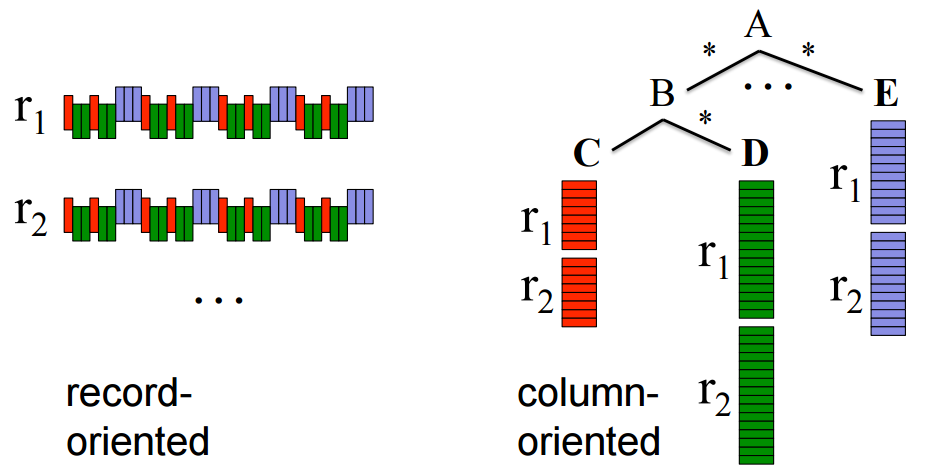
\includegraphics[width=\linewidth]{columnar.png}
\end{columns}

\vspace{0.5 cm}
I don't think it would make sense to use Parquet's definition and repetition levels:
\begin{center}
\textcolor{blue}{\scriptsize\url{https://blog.twitter.com/2013/dremel-made-simple-with-parquet}}
\end{center}
since the repetition levels can't be interpreted independently: you need to know the elements' neighbors to know how to interpret them.

\vspace{0.2 cm}
Also, they take too much memory: every repeated field requires a repetition level array, though the fields of a repeated record would have identical repetition levels.
\end{frame}

\begin{frame}{Data representation}
\vspace{0.5 cm}
Instead, link columns of different levels (e.g.\ event level and particle level) with two short arrays at the outer level: first index and number of elements. These can be shared among all fields of a record in a variable-sized collection.

\vspace{0.25 cm}
\textcolor{darkblue}{\bf Example:}

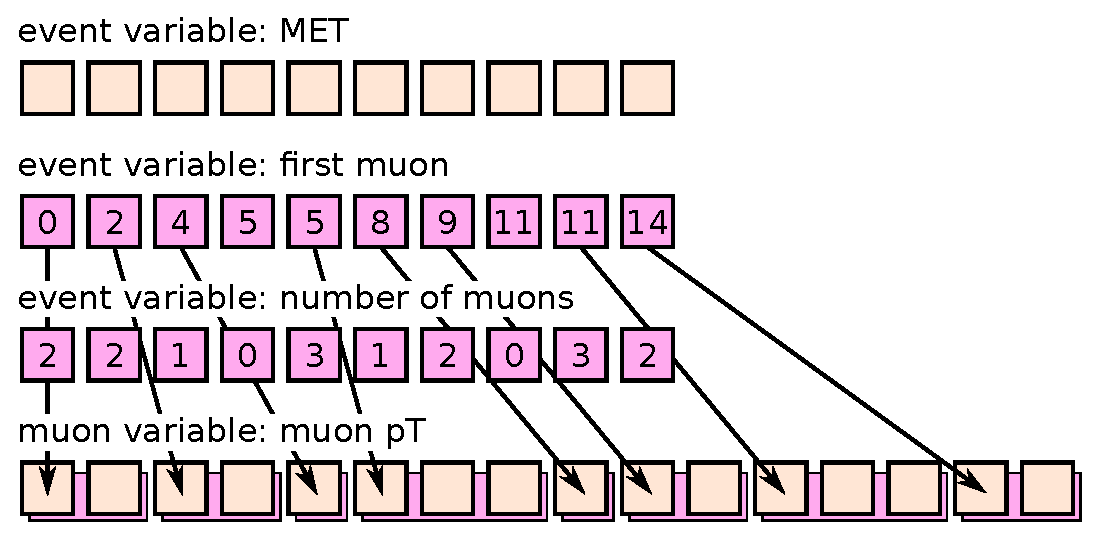
\includegraphics[width=\linewidth]{hierarchical_arrays.pdf}
\end{frame}

\begin{frame}{Status}
\vspace{0.25 cm}
\small
\begin{columns}[t]
\column{0.5\linewidth}
\begin{tabular}{r >{\raggedright}p{0.6\linewidth} c}
& step & done? \\\hline
1 & syntax BNF & $\surd$ \\
2 & parser & $\surd$ \\
3 & typeless AST & $\surd$ \\
4 & assignments and user-defined functions & $\surd$ \\
5 & variable shadowing & $\surd$ \\
6 & type system & $\surd$ \\
7 & type $\cup$, $\cap$, $\backslash$ & $\surd$ \\
8 & type inference & $\surd$ \\
9 & type constraints (``if'', ``and'', ``or'') & $\surd$ \\
10 & type propagation through operators & $\surd$ \\
11 & type propagation through other functions & \textcolor{red}{no} \\
12 & typed AST & $\surd$ \\
13 & collate identical expressions & $\surd$ \\
\end{tabular}

\column{0.5\linewidth}
\begin{tabular}{r >{\raggedright}p{0.6\linewidth} c}
& step & done? \\\hline
14 & expressions to statements & \textcolor{red}{no} \\
15 & generate intermediate representation & \textcolor{red}{no} \\
16 & simple Numpy implementation & \textcolor{red}{no} \\
17 & focus group syntax, user interface & \textcolor{red}{no} \\
18 & discuss with Philippe & \textcolor{red}{no} \\
19 & start integrating into Terascope & \textcolor{red}{no} \\
20 & implement example of each level-changing function & \textcolor{red}{no} \\
21 & GPU development with Peter Hansen & \textcolor{red}{no} \\
22 & big library of functions & \textcolor{red}{no} \\
23 & regular development & \textcolor{red}{no} \\
\end{tabular}
\end{columns}
\end{frame}

\end{document}
